\documentclass[onecolumn, draftclsnofoot,10pt, compsoc]{IEEEtran}
\usepackage{graphicx}
\usepackage[section]{placeins}
\usepackage{url}
\usepackage{setspace}
 
\usepackage{alltt}                                           
\usepackage{float}
\usepackage{color}
\usepackage{url}

\usepackage{geometry}
\geometry{textheight=9.5in, textwidth=7in}
\setlength\parindent{0pt}

% 1. Fill in these details
\def \CapstoneTeamName{\textbf{Insert Team Name Here} }
\def \CapstoneTeamNumber{8}
\def \GroupMemberOne{James Stallkamp}
\def \GroupMemberTwo{Jeremy Fischer}
\def \GroupMemberThree{Austin Row}
\def \CapstoneProjectName{NLP For Digital Manufacturing}
\def \CapstoneSponsorCompany{Autodesk}
\def \CapstoneSponsorPerson{Patti Vrobel}
\def \botname{Aviato }
\def \totalMemoryRequirement{20 MB }

% 2. Uncomment the appropriate line below so that the document type works
\def \DocType{		%Problem Statement
				Requirements Document
				%Technology Review
				%Design Document
				%Progress Report
				}
			
\newcommand{\NameSigPair}[1]{\par
\makebox[2.75in][r]{#1} \hfil 	\makebox[3.25in]{\makebox[2.25in]{\hrulefill} \hfill		\makebox[.75in]{\hrulefill}}
\par\vspace{-12pt} \textit{\tiny\noindent
\makebox[2.75in]{} \hfil		\makebox[3.25in]{\makebox[2.25in][r]{Signature} \hfill	\makebox[.75in][r]{Date}}}}
% 3. If the document is not to be signed, uncomment the RENEWcommand below
\renewcommand{\NameSigPair}[1]{#1}

%%%%%%%%%%%%%%%%%%%%%%%%%%%%%%%%%%%%%%%
\begin{document}
\begin{titlepage}
    \pagenumbering{gobble}
    \begin{singlespace}
    	
\includegraphics[height=4cm]{coe_v_spot1}
        %\hfill 
        % 4. If you have a logo, use this includegraphics command to put it on the coversheet.
        
\includegraphics[height=4cm]{autodesk}   
        \par\vspace{.2in}
        \centering
        \scshape{
            \huge CS Capstone \DocType \par
            {\large\today}\par
            \vspace{.5in}
            \textbf{\Huge\CapstoneProjectName}\par
            \vfill
            {\large Prepared for}\par
            \Huge \CapstoneSponsorCompany\par
            \vspace{5pt}
            {\Large\NameSigPair{\CapstoneSponsorPerson}\par}
            {\large Prepared by }\par
            Group\CapstoneTeamNumber\par
            % 5. comment out the line below this one if you do not wish to name your team
            %\CapstoneTeamName\par 
            \vspace{5pt}
            {\Large
                \NameSigPair{\GroupMemberOne}\par
                \NameSigPair{\GroupMemberTwo}\par
                \NameSigPair{\GroupMemberThree}\par
            }
            \vspace{20pt}
        }
        \begin{abstract}
       		This document outlines the technical requirements of \botname that \CapstoneProjectName must meet. This document starts with an overall description of the project followed by specific functional and performance requirements and ends with a Gantt chart which gives a rough timeline of when each major requirement shall be done.
        \end{abstract}     
    \end{singlespace}
\end{titlepage}
\newpage
\pagenumbering{arabic}
\tableofcontents
% 7. uncomment this (if applicable). Consider adding a page break.
%\listoffigures
%\listoftables
\clearpage

% 8. now you write!
\section{Introduction}
        The introduction outlines the purpose and scope of the project. 
        This section is responsible for defining any prerequisite acronyms and terms used in the document. 
    \subsection{Purpose}
        The purpose of this document is to lay out the requirements of \CapstoneTeamName. 
        This document is a mutual agreement between both parties outlining what will be produced. 
        The intended audience is those who will be working on \CapstoneTeamName and the client for whom \CapstoneTeamName is for.
    \subsection{Scope}
        \botname will be a speech-based virtual assistant for Fusion 360 that lets users perform any one of a subset of tasks within the product, such as saving a document or opening a menu, by verbally instructing it to perform the task.
        Workflows in Fusion 360 that are not suited for handling by a voice interface will not be supported by \botname.
        As a stretch goal, \botname will be capable of questioning user and storing responses to use to predict and automatically assist with future user behavior.
        It will be a plugin that is bundled with Fusion 360 and will be part of the product's standard download.

        \botname will offer users a tool that decreases the time required to achieve their goals within Fusion 360 by offering an interface that runs in parallel with and complements the keyboard and mouse.
        If the stretch goal is achieved, \botname will further increase productivity by learning to predict and automate specific workflows within the product.
        

    \subsection{Definitions, Acronyms, and Abbreviations}
        \begin{table}[h]
            \centering
            \caption{Definitions}
            \label{my-label}
            \begin{tabular}{|l|l|}
                \hline
                \textbf{Term} & \textbf{Definition} \\ \hline
                API & Application programing interface \\ \hline
                CAD & Computer Aided Design \\ \hline
                CAM & Computer Aided Manufacturing \\ \hline
                Fusion 360 & 
                Referred to as just, Fusion, is an Autodesk Cloud-based 3D CAD/CAM tool/product \\ \hline
                Task & In the context of Fusion 360, a function or operation that can be performed in Fusion 360 \\ \hline
                Plugin & Software that adds specific new functionlity to another piece of software \\ \hline
                User & Someone who interacts \botname  \\ \hline
                Workflow & A sequence of tasks \\ \hline
            \end{tabular}
        \end{table}
    %\subsection{References}
        %TODO
    \subsection{Overview}
        %This section describes the contents and organization of the rest of the document. 
        The rest of this document contains a user story outlining intended uses and specific functionalities of \botname as well as assumptions, dependencies, and design constraints. 

\section{Overall Description}
    \subsection{Product Perspective}

        %\subsubsection{System Interfaces}
            %TODO: Revisit this. I'm not sure if it is applicable to this project.
        \subsubsection{User Interfaces}
            The user will interact with \botname via voice commands spoken in English. 
            In the case of the stretch goal, \botname will periodically speak back to the user to receive insights into the user's actions.

        \subsubsection{Hardware Interfaces} %Included above in the User Interfaces section
            \botname will be supported on desktop and laptop computers that support Fusion 360 and have microphones to receive the user's speech.
            For stretch goal support, devices will also need speakers through which \botname can speak back to the user.
            %TODO: Any other devices? Is there anything else that supports Fusion?

        \subsubsection{Software Interfaces}               
            %TODO: Should the API version/specific open source projects being used be added here?
            \botname needs to translate supported speech commands received from the user to the equivalent tasks within the user's Fusion project.
            The Fusion source code will not be available for modification, thus the commands will need to be executed via the existing Fusion API.
            To translate the commands, the audio recorded by the user interface will need to be processed by a speech-to-text application.
            The resulting output will need to be parsed by another application that can derive meaning from natural language text.
            Finally, the derived meaning will need to have a deterministic mapping to a Fusion API call and thus to a specific task inside of Fusion.
            %TODO: Insert block diagram here.
            %TODO: Describe software interfaces for stretch goal where UI communicates back to user then stores/uses responses
        %\subsubsection{Communications Interfaces}                

        \subsubsection{Memory} 
            \botname will require at most \totalMemoryRequirement of memory to perform the work necessary to add its functionality to Fusion.
            For the stretch goal of storing data related to user responses to questions from \botname, there are no memory caps at this time on the amount of data that can be stored.

        %\subsubsection{Operations}
            %TODO: I'm not sure what this section means.

        \subsubsection{Site Adaptation Requirements} 
            Since \botname interacts with Fusion using existing architecture, Fusion will not need to be modified to support it. 

    \subsection{Product Functions}
        \botname will allow the user to perform tasks in Fusion via a voice interface. 
        Each voice command given by the user will be mapped to a specific task which will then be performed in the open Fusion project. \\
       
        As a stretch goal, \botname will periodically ask the users questions regarding why they have performed specific tasks.
        The questions asked by \botname will pertain to specific predefined contexts.
		\botname will record user responses and save a transcript along with contextual information.
        
    \subsection{User Characteristics}
		\botname will have two types of users: administrators and designers. 
		Administrators will have access to data collected by \botname including the command logs and, if the stretch goal is accomplished, user responses to questions from \botname. 
		
		The primary user is the designer who is working on projects inside of Fusion. 
        Due to the technical knowledge needed to work within Fusion, it can be assumed that designers are technically oriented.
        However, no extra knowledge outside of that needed to operate Fusion will be needed to operate \botname.
        
    \subsection{Constraints}
        \botname will not be integrated to with the Fusion source code and thus will be constrained in what tasks it can perform by what is offered in the Fusion API. 

    \subsection{Assumptions and Dependencies}
        The stretch goal assumes that the Fusion API offers a way to view actions the user performs with their keyboard and mouse.
        Without this capability, the application's knowledge of user actions will be limited to the actions that the user performs through \botname.

\section{Specific Requirements}
    \subsection{External Interface}
       First time users of \botname will be presented with an onboarding process with an interactive demo.
       The onboarding process will start with a popup that introduces \botname with a concise description of its purpose.
       The user will then be able to click "Next" to transition to an interactive demo.
       The interactive demo will consist of several sequential popups that each ask the user to tell \botname to perform a specific command.
       This will make the user aware of \botname and the functionality that it offers.

    \subsection{Functional Requirements}
    This section includes the requirements that specify all the fundamental actions of the software system.
        \subsubsection{Functional Requirement 1}
        TITLE: Error Messaging \\
        DESCRIPTION: The system shall alert the user when it cannot perform or does not understand a command. \\
        RATIONAL: If a user's command is not executed, they must be informed why. 
        
        \subsubsection{Functional Requirement 2}
        TITLE: Correspond voice command to Fusion 360 action  \\
        DESCRIPTION: The system shall be able to correspond the produced text equivalent described in FR1 to the correct Fusion action. \\
        RATIONAL: This must be done to run commands in Fusion 
        
        \subsubsection{Functional Requirement 3}
        TITLE: Send commands to Fusion  \\
        DESCRIPTION: The system shall be able to send the generated action from FR2 to Fusion. \\
        RATIONAL: This is the last step in the voice command to Fusion action pipeline 
        
        \subsubsection{Functional Requirement 4}
        TITLE: Extrude \\
        DESCRIPTION: \botname shall be able to extrude a selected face. \\
        RATIONAL: This is a task that users perform often.
        
        \subsubsection{Functional Requirement 5}
        TITLE: Rotate Camera \\
        DESCRIPTION: \botname shall be able to rotate the Fusion camera. \\
        RATIONAL: This is a task that users perform often.
        
        \subsubsection{Functional Requirement 6}
        TITLE: Save Project \\
        DESCRIPTION: \botname shall be able to save a Fusion project. \\
        RATIONAL: This is a task that users perform often.
        
        \subsubsection{Functional Requirement 7}
        TITLE: Logging User Interactions \\
        DESCRIPTION: \botname shall log every interaction that a user has with \botname and the result of that interaction. \\
        RATIONAL: This offers helpful information for debugging purposes. This information can also be used to learn how \botname is being used and for directing future development of \botname.
        
        %	%
        %	Below are stretch goals
        %	%
        
        \subsubsection{Stretch Functional Requirement 1}
        TITLE: What interview question to ask \\
        DESCRIPTION: The system shall be able to generate an interview question. \\
        RATIONAL: This is the first step in collecting user reasoning data.  
        
        \subsubsection{Stretch Functional Requirement 2}
        TITLE: When to ask an interview question \\
        DESCRIPTION: The system shall be aware of when it is appropriate to ask a question. \\
        RATIONAL: This is the second step in collecting user reasoning data. 
        
        \subsubsection{Stretch Functional Requirement 3}
        TITLE: Ask a question \\
        DESCRIPTION: The system shall be able to ask a question to the user. \\
        RATIONAL: This is the third step in collecting user reasoning data. 
        
        \subsubsection{Stretch Functional Requirement 4}
        TITLE: Output interview text to a file \\
        DESCRIPTION: The system shall be able to output an interview question paired with the user's answer to a file. \\
        RATIONAL: This is the last step in collecting user reasoning data. 
        

    \subsection{Performance Requirements}
        The section lists the performance requirements that will be met by \botname.
        
        \subsubsection{Performance Requirement 1}
        TITLE: Supported Number of Simultaneous Users \\
        DESCRIPTION: There is no limit on the number of users, but \botname will only process one command at time and thus will ignore commands given simultaneously. \\
        RATIONAL: It is difficult to separate two commands when they are given simultaneously and is considered beyond the scope of this project.
        
        \subsubsection{Performance Requirement 2}
        TITLE: \botname Response Time \\
        DESCRIPTION: A call to the Fusion API shall be initiated within one a second of \botname hearing a valid command from the user. \\
        RATIONAL: This is considered the maximum reponse time of a user interface to ensure the user maintains their thought process and is not distracted by the interface.
        
    \subsection{Design Constraints}
        \botname will execute tasks in Fusion via the Fusion API. 
        Therefore supported tasks will constrained to those capable of being performed by the API.
        
    \subsection{Software System Attributes}
	   	\subsubsection{Reliability}
	   	SCALE: \botname executes supported voice commands when they are given. 
	   	METER: Measurements obtained from 10 trials per supported command.\\
	   	MUST: Execute supported command in at least 70\% of trials.\\
	   	PLAN: Execute supported command in at least 80\% of trials.\\
        WISH: Execute supported command in at least 90\% of trials.\\
   
\section{Release Plan}
	The develop of \botname is very sequential. Each step's development and success depends on how the previous step was implemented. For that reason, \CapstoneProjectName's release plan remains tentative. Below is a Gantt chart outlining \botname's development plan.
    \subsection{Release plan}
    	\begin{figure}[H]
    		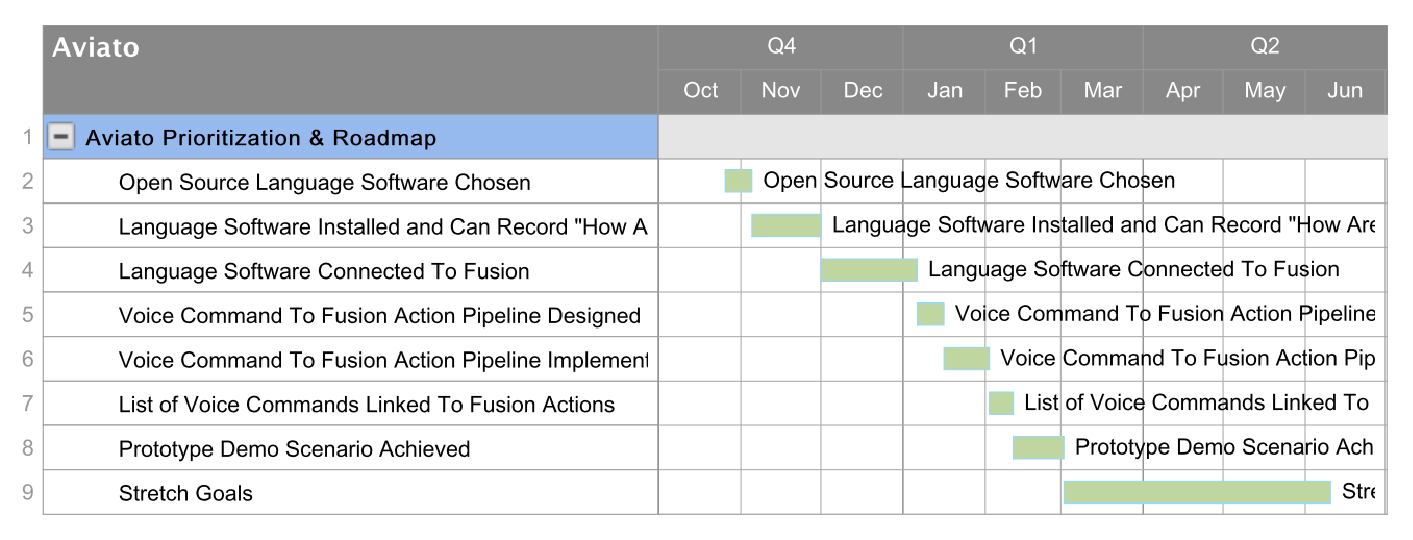
\includegraphics[width=1\textwidth]{ganttChart.eps}
    		\centering
    		\caption{\botname Development Schedule}
   			\label{fig:developmentSchedule1}
    	\end{figure}


%\bibliography{requirementsBib} 
%\bibliographystyle{ieeetr}

\end{document}
